\appendix
\section{Appendix}
\subsection{Varying the parameters of the Aliev \& Panfilov model}
\label{app:ap-params}

\begin{figure}[h]
    \centering
    \begin{subfigure}[b]{\textwidth}
        \includegraphics[width=\textwidth]{alpha-params-1}
        \vspace{-2\baselineskip}
        \caption{a}
    \end{subfigure}
    \begin{subfigure}[b]{\textwidth}
        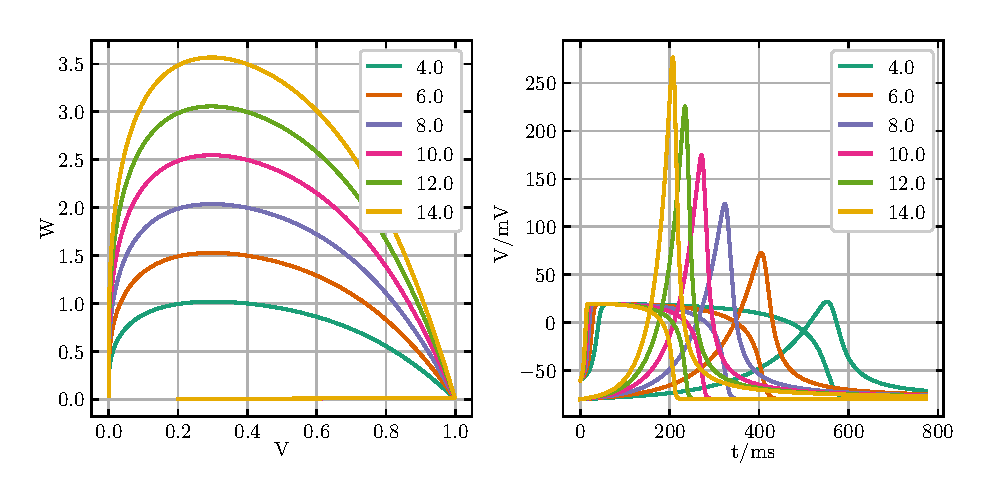
\includegraphics[width=\textwidth]{alpha-params-2}
        \vspace{-2\baselineskip}
        \caption{k}
    \end{subfigure}
    \begin{subfigure}[b]{\textwidth}
        \includegraphics[width=\textwidth]{alpha-params-3}
        \vspace{-2\baselineskip}
        \caption{$\epsilon_0$}
    \end{subfigure}
\end{figure}
\begin{figure}[h]
    \ContinuedFloat
    \centering
    \begin{subfigure}[b]{\textwidth}
        \includegraphics[width=\textwidth]{alpha-params-4}
        \vspace{-2\baselineskip}
        \caption{$\mu_1$}
    \end{subfigure}
    \begin{subfigure}[b]{\textwidth}
        \includegraphics[width=\textwidth]{alpha-params-5}
        \vspace{-2\baselineskip}
        \caption{$\mu_2$}
    \end{subfigure}
    \label{app:ap-params}
    \caption{}
\end{figure}

% vim: set ff=unix tw=79 sw=4 ts=4 et ic ai :
